\documentclass{article}
\usepackage[backend=biber,natbib=true,style=authoryear,maxbibnames=10]{biblatex}
\addbibresource{/home/nqbh/reference/bib.bib}
\usepackage[utf8]{vietnam}
\usepackage{tocloft}
\renewcommand{\cftsecleader}{\cftdotfill{\cftdotsep}}
\usepackage[colorlinks=true,linkcolor=blue,urlcolor=red,citecolor=magenta]{hyperref}
\usepackage{amsmath,amssymb,amsthm,float,graphicx,mathtools,tikz}
\allowdisplaybreaks
\newtheorem{assumption}{Assumption}
\newtheorem{baitoan}{Bài toán}
\newtheorem{cauhoi}{Câu hỏi}
\newtheorem{conjecture}{Conjecture}
\newtheorem{corollary}{Corollary}
\newtheorem{dangtoan}{Dạng toán}
\newtheorem{definition}{Definition}
\newtheorem{dinhly}{Định lý}
\newtheorem{dinhnghia}{Định nghĩa}
\newtheorem{example}{Example}
\newtheorem{ghichu}{Ghi chú}
\newtheorem{hequa}{Hệ quả}
\newtheorem{hypothesis}{Hypothesis}
\newtheorem{lemma}{Lemma}
\newtheorem{luuy}{Lưu ý}
\newtheorem{nhanxet}{Nhận xét}
\newtheorem{notation}{Notation}
\newtheorem{note}{Note}
\newtheorem{principle}{Principle}
\newtheorem{problem}{Problem}
\newtheorem{proposition}{Proposition}
\newtheorem{question}{Question}
\newtheorem{remark}{Remark}
\newtheorem{theorem}{Theorem}
\newtheorem{vidu}{Ví dụ}
\usepackage[left=1cm,right=1cm,top=5mm,bottom=5mm,footskip=4mm]{geometry}
\def\labelitemii{$\circ$}
\DeclareRobustCommand{\divby}{%
	\mathrel{\vbox{\baselineskip.65ex\lineskiplimit0pt\hbox{.}\hbox{.}\hbox{.}}}%
}

\title{TikZ}
\author{Nguyễn Quản Bá Hồng\footnote{Independent Researcher, Ben Tre City, Vietnam\\e-mail: \texttt{nguyenquanbahong@gmail.com}; website: \url{https://nqbh.github.io}.}}
\date{\today}

\begin{document}
\maketitle
\begin{abstract}
	A personal practice of drawing figures in \LaTeX\ by using TikZ package.
\end{abstract}
\tableofcontents
\newpage

%------------------------------------------------------------------------------%

\section{Hệ Trục Tọa Độ}
See \cite{Quy2022}.

\begin{center}
	\begin{tikzpicture}[>=stealth,scale=.75]
		\draw[->](-3,0)--(3,0) node[above]{$x$};
		\draw[->](0,-3)--(0,3) node[left]{$y$};
		\draw[dashed](0,1)--(2,1)--(2,0);
		\draw(2,1) circle(0.05) node[above right]{$A$};
		\path(0,0) node [below left]{$O$};
	\end{tikzpicture}
\end{center}

%------------------------------------------------------------------------------%

\section{Vẽ Điểm}

\begin{center}
	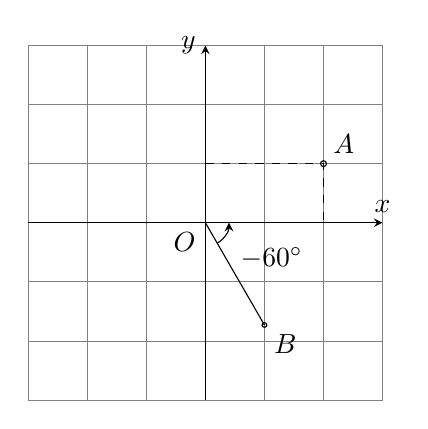
\begin{tikzpicture}[>=stealth,scale=.75]
		\draw[step=1,gray,very thin](-3,-3) grid (3,3);
		\draw[->](-3,0)--(3,0);
		\draw[->](0,-3)--(0,3);
		\draw[dashed](0,1)--(2,1)--(2,0);
		\draw(2,1) circle(.05);
		\draw(3,0) node[above]{$x$} (0,3) node[left]{$y$} (0,0) node[below left]{$O$};
		\draw(-60:2) circle(0.04);
		\draw(-60:2) -- (0,0);
		\draw(2,1) node[above right]{$A$} (-60:2) node[below right]{$B$};
		\draw[->](-60:4mm) arc(-60:0:4mm);
		\path(-30:5mm) node[below right]{$-60^\circ$};
	\end{tikzpicture}
\end{center}

%------------------------------------------------------------------------------%

\printbibliography[heading=bibintoc]
	
\end{document}